\documentclass[twocolumn]{article}  %define file type and 
\usepackage[sc]{mathpazo} % Use the Palatino font
\usepackage[T1]{fontenc} % Use 8-bit encoding that has 256 glyphs
\linespread{1.15} % Line spacing - Palatino needs more space between lines
\usepackage{microtype} % Slightly tweak font spacing for aesthetics
\usepackage[english]{babel} % Language hyphenation and typographical rules
\usepackage{graphicx}
%\usepackage[hmarginratio=1:1,top=32mm,columnsep=20pt]{geometry} % Document margins
%\usepackage[hmarginratio=1:1,top=30mm,columnsep= 6pt]{geometry} 
\usepackage[left=1.2cm,right=1.2cm,top=2cm,columnsep= 20pt]{geometry}
\usepackage[hang, small,labelfont=bf,up,textfont=it,up]{caption} % Custom captions under/above floats in tables or figures
\usepackage{booktabs} % Horizontal rules in tables
\usepackage{amsmath}
\usepackage{enumitem} % Customized lists
\setlist[itemize]{noitemsep} % Make itemize lists more compact
\usepackage{abstract} % Allows abstract customization
\renewcommand{\abstractnamefont}{\normalfont\bfseries} % Set the "Abstract" text to bold
\renewcommand{\abstracttextfont}{\normalfont\small\itshape} % Set the abstract itself to small italic text
\usepackage{subfigure}
\usepackage{titlesec} % Allows customization of titles
\setcounter{secnumdepth}{4}
\titleformat{\paragraph}
{\normalfont\normalsize\bfseries}{\theparagraph}{1em}{}
\titlespacing*{\paragraph}
%{0pt}{3.25ex plus 1ex minus .2ex}{1.5ex plus .2ex}
{0pt}{1ex minus .2ex}{1.5ex plus .2ex}
\usepackage{fancyhdr} % Headers and footers
\pagestyle{fancy} % All pages have headers and footers
\fancyhead{} % Blank out the default header
\fancyfoot{} % Blank out the default footer
\fancyfoot[RO,LE]{\thepage} % Custom footer text
\pagestyle{plain}
\usepackage{titling} % Customizing the title section
\usepackage{hyperref} % For hyperlinks in the PDF
\usepackage{indentfirst}
\usepackage{mathrsfs}
\usepackage{booktabs} %??????{booktabs}
\usepackage{rotating}
\newsavebox{\tablebox}
\usepackage{adjustbox}
%\usepackage[page,title,titletoc,header]{appendix}
\usepackage{float} %???????????
\usepackage{subfigure} %?????????????
\renewcommand\thesection{\Roman{section}}  
\renewcommand\thesubsection{\Alph{subsection}}
\usepackage{amsmath}
\usepackage{autobreak}
\usepackage{amssymb}
\usepackage{caption}
\usepackage{algorithm}
\usepackage{algorithmicx}
\usepackage{algpseudocode}
\usepackage{amsmath}
\renewcommand{\algorithmicrequire}{\textbf{Input:}}  % Use Input in the format of Algorithm
\renewcommand{\algorithmicensure}{\textbf{Output:}} % Use Output in the format of Algorithm
\setlength\parindent{0pt}

%----------------------------------------------------------------------------------------
%	TITLE SECTION
%----------------------------------------------------------------------------------------

\setlength{\droptitle}{-4\baselineskip} % Move the title up
\pretitle{\begin{center}\Huge\bfseries} % Article title formatting
%\pretitle{\begin{center}\Huge}
\posttitle{\end{center}} % Article title closing formatting
\title{Image and Video Compression Laboratory\\Outline of implemented Techniques} % Article title
\author{
\scriptsize Yanchen Huang\\[1ex] 
\scriptsize Technical University of Munich\\ % Your institution
\scriptsize Matrikel-Nr: 03715208\\ % Your institution
\scriptsize {Email: yanchen.huang@tum.de}\\ % Your email address
\and % Uncomment if 2 authors are required, duplicate these 4 lines if more
\scriptsize Chang Liu\\[1ex] 
\scriptsize Technical University of Munich\\ % Your institution
\scriptsize Matrikel-Nr: 03707882\\ % Your institution
\scriptsize {Email: ge29ney@tum.de}\\ 
}
\date{}

%----------------------------------------------------------------------------------------

\begin{document}\small
% Print the title
\maketitle
%\thispagestyle{empty}
%----------------------------------------------------------------------------------------
%	ARTICLE CONTENTS
%----------------------------------------------------------------------------------------
%\newpage
%\thispagestyle{empty}
%\tableofcontents
%\newpage
%\setcounter{page}{1}

%\begin{enumerate}
%\item 
%\end{enumerate}

%%%%%%%%%%%%%%%%%%%%%%%%%%%%%%%%%%%%%%%%%%
\section{Introduction}
%%%%%%%%%%%%%%%%%%%%%%%%%%%%%%%%%%%%%%%%%%
Optimization methods: PCA for color space conversion, deblocking filter, DWT and SPIHT algorithm are implemented in our project and explained in detail in this outline. 
%The comparison of the results between the baseline and the optimization techniques are presented in the last chapter.
%%%%%%%%%%%%%%%%%%%%%%%%%%%%%%%%%%%%%%%%%%
\section{Color Space Conversion: PCA }
%%%%%%%%%%%%%%%%%%%%%%%%%%%%%%%%%%%%%%%%%%
Conversion between RGB and YCbCr usually follows ITU-R BT.601 standard, which is a fixed space conversion matrix. However, different images have different color properties, to preserve more color information for each image, a better conversion algorithm such as PCA is needed.
Based on the reference paper, "A better Color Space Conversion Based on Learned Variances For Image Compression\cite{PCA}", an optimal RGB-YCbCr convert matrix for each image is defined in equation \eqref{eq1} as $T_{enc}$ and $Offset_{enc}$.
\begin{equation}
\left[
\begin{array}{ccc}
Y \\
Cb\\
Cr
\end{array}
\right]=
\left[
\begin{array}{ccc}
x1 & x2 & x3   \\
y1 & y2 & y3   \\
z1 & z2 & z3
\end{array}
\right]
\left[
\begin{array}{ccc}
R  \\
G  \\
B
\end{array}
\right]
+
\left[
\begin{array}{ccc}
Y\_offset \\
Cb\_offset \\
Cr\_offset
\end{array}
\right]\label{eq1}
\end{equation}
Each row in $T_{enc}$ is the direction of the new YCbCr space's base axis, to find the optimal axis, PCA is applied. Firstly, the whole picture is divided into 8*8 grids, each pixel in the grid should minus the mean value within the same grid. Secondly, covariance matrix of size 3*3 is computed and PCA is utilized to find eigenvalues and eigenvectors. Stack the eigenvectors based on the descend order of the corresponding eigenvalues to form our $T_{pca}$ as follow. 
$$
\left[
\begin{array}{ccc}
x_{p}1 & x_{p}2 & x_{p}3   \\
y_{p}1 & y_{p}2 & y_{p}3   \\
z_{p}1 & z_{p}2 & z_{p}3
\end{array}
\right]
$$
Thirdly, based on the reference paper, according to YCbCr's range restrictions, scaling is done based on following equation\eqref{eq2}.
\begin{equation}
\begin{aligned}
&\left[x1, x2, x3\right]= L1\_normalize(\left[x_{p}1, x_{p}2, x_{p}3\right])*219/255\\
&Scale_{Cb} := 224/255/(|y_{p}1| + |y_{p}2| + |y_{p}3|) \\
&\left[y1, y2, y3\right] = \left[y_{p}1, y_{p}2, y_{p}3\right]*Scale_{Cb} \\
&Scale_{Cr} := 224/255/(|z_{p}1| + |z_{p}2| + |z_{p}3|) \\
&\left[z1, z2, z3\right] = \left[z_{p}1, z_{p}2, z_{p}3\right]*Scale_{Cr}
\end{aligned}\label{eq2}
\end{equation}
$Offset_{enc}$ is defined as equation\eqref{eq3}.
\begin{equation}
\begin{aligned}
&Y\_offset = 16\\
&Cb\_offset = -1*sum\_negative(y1,y2,y3)*255 + 16\\
&Cr\_offset = -1*sum\_negative(z1,z2,z3)*255 + 16\
\end{aligned}\label{eq3}
\end{equation}
In decoding, instead of using $T_{enc}^{-1}$, $T_{dec}$ is computed through least square method, i.e. linear regression. The convert formula is shown in equation\eqref{eq4}.
\begin{equation}
\left[
\begin{array}{ccc}
R\\
G\\
B
\end{array}
\right]=
T_{dec}*(
\left[
\begin{array}{ccc}
Y  \\
Cb  \\
Cr
\end{array}
\right]
-
\left[
\begin{array}{ccc}
Y\_offset \\
Cb\_offset \\
Cr\_offset
\end{array}
\right])
\label{eq4}
\end{equation}
To further optimize the result, polynomial curve fitting is applied to the converted RGB image, i.e. use converted RGB image and original RGB image to train coefficient for a polynomial mapping of degree 3 to find the best match.
%%%%%%%%%%%%%%%%%%%%%%%%%%%%%%%%%%%%%%%%%%
\section{Deblocking filter}
%%%%%%%%%%%%%%%%%%%%%%%%%%%%%%%%%%%%%%%%%%
Deblocking filter is applied to reduce blocking distortion by smoothing the block edges. Based on H.264/AVC Loop filter\cite{deblock}, we first take vertical and horizontal edges of 8*8 macroblock as depicted in Fig.~\ref{fig:0}. \\
\\
\\
\begin{figure}[h]
\centering
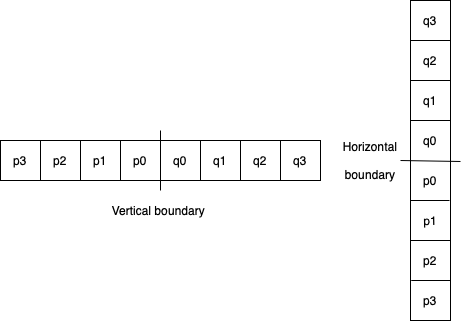
\includegraphics[scale=0.45]{boundary.png}
\caption{Pixels adjacent to vertical and horizontal boundaries}
\label{fig:0}
\end{figure}\\
Secondly, to determine the true boundary for applying deblock filter, two conditions shown as follow should be fulfilled, notice that in our project, thresholds $\alpha$ and $\beta$ are prefixed.
\begin{itemize}
\item |p0 - q0| < $\alpha$
\item |p1 - q1| < $\beta$
\end{itemize}
Thirdly, a 4-tap linear filter is applied with inputs p1, p0, q0, q1 if the filter is applicable. Output value would be assigned to position p0 and q0 as the new value for the filtered boundary. 

%%%%%%%%%%%%%%%%%%%%%%%%%%%%%%%%%%%%%%%%
\section {Sparsity based adaptive quantization}
%%%%%%%%%%%%%%%%%%%%%%%%%%%%%%%%%%%%%%%%   
The basic idea of this algorithm is using the sparsity of the image to adptively choose the quantization table, namely the qScale. The sparsity shows the detail distribution in each area of the image. The sparsity can be determined by the larger parameters of each DCT Block. 
\\
The SparsityMap is determined by counting the number of larger parameters in each DCT block.
\begin{algorithm}[h]  
  \caption{: determine the Sparsity}
	\begin{algorithmic}
	\Require
      the blockwise DCT transformed image  $I_{DCT}$;
    \Ensure
     	 $SparsityMap$ for the $I_{DCT}$;
	\State
	\For{$Block_{ij} \in I_{DCT}$}
      \State Threshold=GAMMA$\times$Max coefficient in DCT Block;
      \State N= numel(coefficients$\geqslant$threshold);
	\State SparityMap(i,j)=N;
    \EndFor	
	\end{algorithmic}
\end{algorithm} 

The value GAMMA is image specific. In this paper I take the GAMMA value as 0.015 for the Foreman video sequence.  
According to the SparsityMap it is shown, that which block contains more details. It means that the greater the number in SparsityMap is, the more details information that block has. \\
Then the quantization scale can be adptively chosen according to the SparsityMap. The basic concept is:

\begin{algorithm}[h]  
  \caption{:determine the qScale}
	\begin{algorithmic}
	\Require
      The $SparsityMap$;
      the qScale baseline $qScale$;
    \Ensure
     	 Suitable qScale $qScale_{new}$ for each individual Block;
	\State
	find the maximum value $S_{max}$ in $SparsityMap$; 
	\For{$SparsityMap_{ij} \in SparsityMap$}
	\State chose the suitable stepsize  $\Delta$ of $qScale$;
     \State $steps$=$SparsityMap_{ij}$/($S_max$$\times$(1/8));
	\State $qScale_{new}$= $qScale$+$\Delta$$\times$$(4-steps)$;
    \EndFor	
	\end{algorithmic}
\end{algorithm} 
The $SparsityMap$ tells us how much detailed information is contained in each block. And we totally divide them into 8 levels(8 contains most detail information).And for the up level, namely $level$ $\in$ [5:8],the quantization factor qScale will be increased. otherwise it will be decreased.     
\\
The other step of the whole compression is basically the same as follow. 

\begin{figure}[ht]
\centering
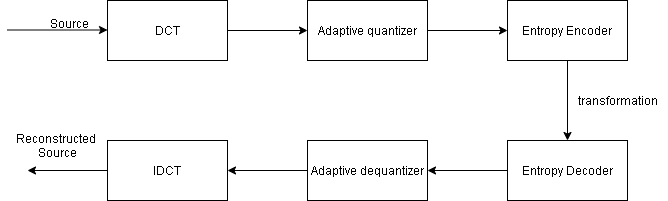
\includegraphics[scale=0.42]{flowDiagram.png}
\caption{DCT based Image/video compression}
\label{fig:1}
\end{figure}

%%%%%%%%%%%%%%%%%%%%%%%%%%%%%%%%%%%%%%%%
\section {DWT-SPIHT based image and video compression}

%%%%%%%%%%%%%%%%%%%%%%%%%%%%%%%%%%%%%%%%
The progress of DWT-SPIHT based image and video compression is very similar to the previous DCT based Compression. The Difference is that instead of dividing the source image to many blocks and do DCT for each block, DWT-SPIHT based compression do n-level DWT for the whole image and quantize them with SPIHT algorithm. 
\subsection{DWT}
when we do the DWT transform we use the $Bior 4.4$ filter.\cite{PCA}The DWT process of the image is as follows.

\begin{algorithm} 
  \caption{:$n$ levels DWT}
	\begin{algorithmic}
	\Require
      The $source image$;
	 filters $Lo_D$,$Hi_D$
    \Ensure
     	 DWT Transformed image $I_{DWT}$;
	\State	
	LL=$source image$;
	\For{$ level \in [1:n]$}
	\State L=$LL$*$Lo_D$;
	\State LL=	(downsampled $L$)*$Lo_D$;
	\State LH=(downsampled $L$)*$Hi_D$;
	\State H=$LL$*$Hi_D$;
	\State HL=	(downsampled $H$)*$Lo_D$;
	\State HH=(downsampled $H$)*$Hi_D$;
	\State Sort each computed part in to $I_{DWT}$.
    \EndFor	
	\end{algorithmic}
\end{algorithm} 
the DWT transformed image will be saved as $I_{DWT}$,which seems like a multi-divided quadrate. and then seems it contains too much coefficient. The $I_{DWT}$ should be quantized and compressed with SPIHT algorithm. The SPIHT algrithm is very similar to EZW algorithm.
  
\subsection {SPIHT algorithm}
The SPIHT algorithm based on EZW algorithm. It applies the same Successive-Approximation Quantization. The main difference of the SPIHT algorithm to EZW algotirhm is that the SPIHT algorithm used a patial orientation tree to more efficiently represent the coefficient structure. The "patial orientation tree" allows it eliminate some root, that for example except the root all the other node are unimportant. 
\begin{algorithm}[t]  
  \caption{:SPIHT algorithm}
	\begin{algorithmic}
	\State \textbf{Initialization} ;
	\State compute Threshol s
	\State LIP=all elements in Tree root
	\State LSP=empty;
	\For{$n\in [1:N]$}
	\State \textbf{Significance Map Encoding(Sorting Pass)}
	\For{$ Coeff(i,j) \in LIP$}
	\State search all coefficient in LIP
	\If {$coefficient\geqslant{threshold}$}
		\State $S_{ij}$=1;
	\Else
		\State $S_{ij}$=0;
	\EndIf
	\State According to the S table fill the LSP Table	
	\EndFor	
	\State \textbf{Process LIS}
	\For{$search all elemet in LIS$}
	\If	{$Type = D$}	
		\State $S_{ij}$= sign($D_{ij}$);
		\If {$S_{ij}=1$}
			\State add item in the LSP list;
		\Else 
			\State add item the LIP list;
		\EndIf
	\Else{$Type = L$}
		\State  $S_{ij}$ = sign($L_{ij}$);

	\EndIf
	\EndFor 
	\State\textbf{Refinement Pass}
	\State \textbf{Process LSP}
	\For{$all\ element\ in\ LSP\ list\ except\ those\ just\ added\ above$}
		\State Output the nth most significant bit of coeff
	\EndFor
	
	\State\textbf{Update};
	\State Update n.
    	\EndFor
	\end{algorithmic}
\end{algorithm} 

 

%----------------------------------------------------------------------------------------
%	REFERENCE LIST
%----------------------------------------------------------------------------------------
\begin{thebibliography}{50} % Bibliography - this is intentionally simple in this template
%\bibitem{MANUAL}       %\cite{MANUAL}
%Virtual Robot Experimentation Platform USER MANUAL\\
%(www.coppeliarobotics.com/helpFiles/index.html)
\bibitem{PCA}   %\cite{PCA}
Li, Manman.  A Better Color Space Conversion Based on Learned Variances For Image Compression. CVPR Workshops (2019).
\bibitem{deblock}   
H.264/AVC Loop Filter. https://www.vcodex.com/h264avc-loop-filter/. Accessed 02.02.2020.
\bibitem {ad_quantization}
Youngjun Yoo Antonio O. and Bin Yu. adptive quantization of image subbands with efficient overhead rate selection.  https://www.researchgate.net/publication/3671825.
Accessed 31.01.2020.
\bibitem {book} K. S. Thyagarajan. Still Image and video compression with Matlab. ISBN 978-0-470-48416-6 
\bibitem {CS} David Fridovich-Keil and Grace Kuo. Compressed Sensing for Image Compression.
\bibitem{JPEG} Gregory Wallace, The JPEG Still Image Compression Standard, 
\bibitem{lecture} Prof. Dr.-Ing. Eckehard Steinbach. Multidimensional signal processing Lecture Skript
\bibitem{SPIHT} SPHIT Algorithm. http://www.ws.binghamton.edu/fowler/fowler$\%$20personal$\%$20page/EE523$\_$files/SPIHT$\_$Charts.pdf. 
\end{thebibliography}
\end{document}
